\begin{figure*}[t]
  \centering
  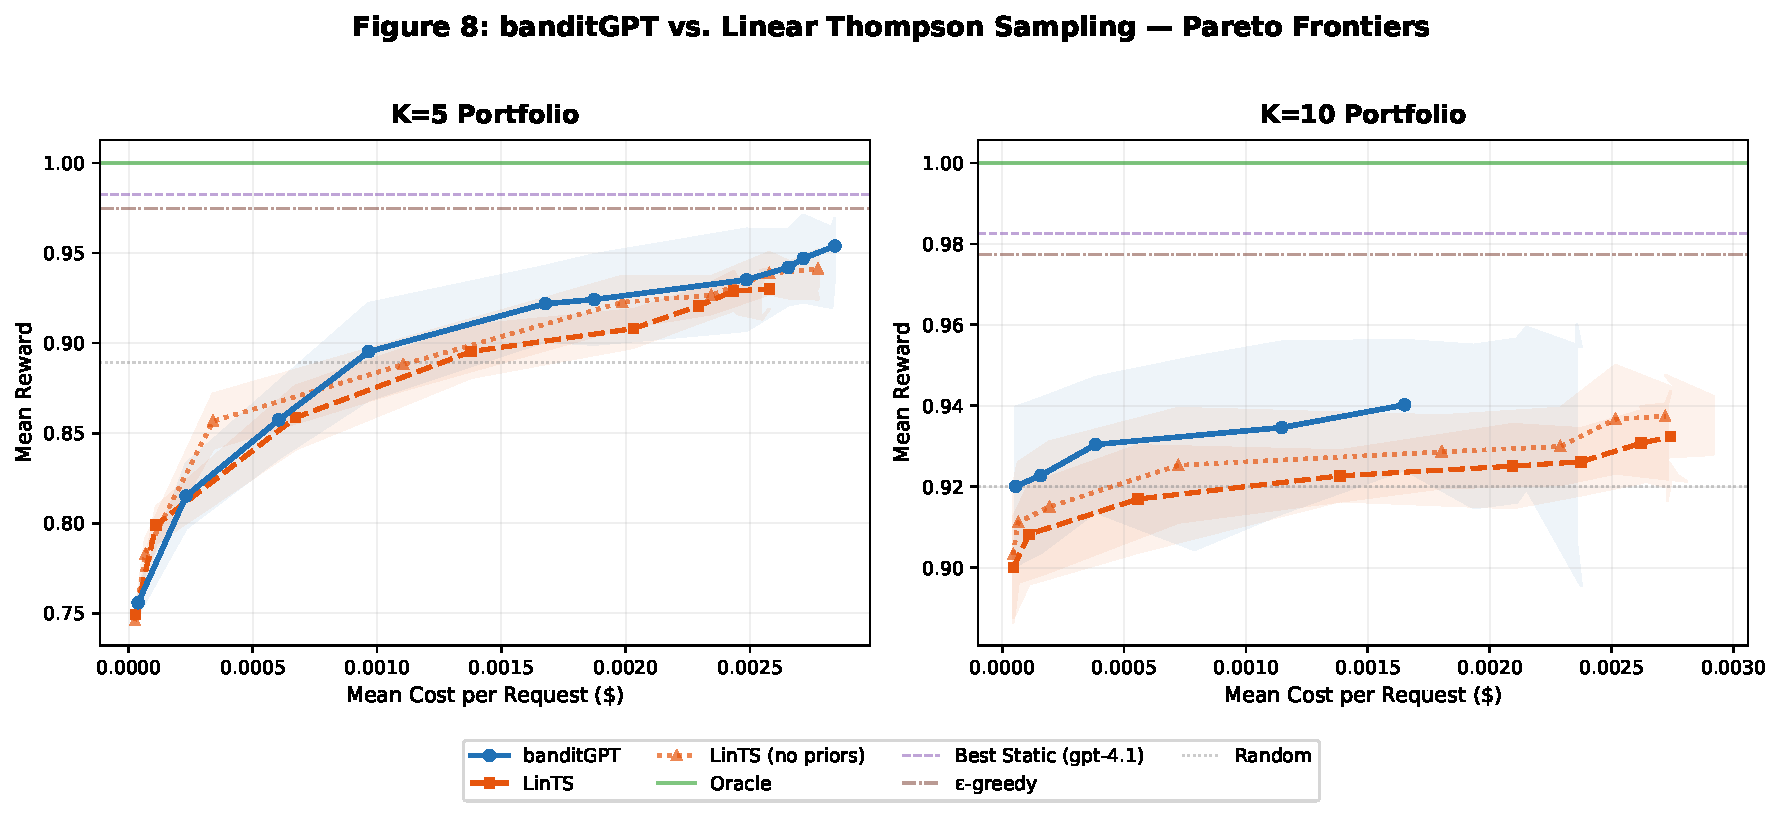
\includegraphics[width=\textwidth]{experiments/07_figure/results/figure8_lints_comparison.pdf}
  \caption{
    \textbf{banditGPT vs.\ Linear Thompson Sampling: Pareto Frontiers at $K{=}5$ and $K{=}10$.}
    Each curve traces the quality--cost Pareto frontier obtained by sweeping the cost-penalty
    parameter $\lambda \in \{0, 0.005, \ldots, 5\}$ across 20 independent trials.
    \emph{Left:} $K{=}5$ portfolio; \emph{Right:} $K{=}10$ portfolio.
    banditGPT (LinUCB + Corralling, solid blue) consistently Pareto-dominates
    LinTS with warmup priors (dashed orange) and LinTS without priors (dotted orange)
    across the full cost spectrum.
    At $K{=}5$, the peak reward gap is 2.4~percentage points
    ($0.954$ vs.\ $0.930$, $p < 0.05$ via paired $t$-test);
    at $K{=}10$ the advantage narrows to 0.8~pp ($0.940$ vs.\ $0.932$).
    Horizontal references show the per-prompt oracle (upper bound),
    best single-model static policy (GPT-4.1), $\varepsilon$-greedy,
    and uniform random baselines.
    Shaded bands denote $\pm 1\sigma$ across trials.
  }
  \label{fig:lints_pareto}
\end{figure*}
